\documentclass[12pt]{article}
\usepackage[utf8]{inputenc}
\usepackage{graphicx}
\usepackage{amsmath}
\usepackage{xcolor}
\usepackage{listings}
\usepackage[margin=1in]{geometry}
\usepackage{hyperref}
\usepackage{caption}
\usepackage{subcaption}
\usepackage{titlesec}
\usepackage{booktabs}
\usepackage{float} % For precise image positioning
\usepackage{afterpage} % For clearing page floats

\definecolor{codebg}{rgb}{0.95,0.95,0.95}
\definecolor{myblue}{rgb}{0,0.3,0.6}

\lstset{
    backgroundcolor=\color{codebg},
    basicstyle=\ttfamily\small,
    breaklines=true,
    frame=single,
    numbers=left,
    numberstyle=\tiny\color{gray},
    keywordstyle=\color{myblue},
    commentstyle=\color{green!50!black},
    stringstyle=\color{red},
    showstringspaces=false,
    tabsize=4
}

\title{Hit-or-Miss Morphological Transformations}
\date{\today}

\begin{document}

\maketitle

\begin{abstract}
This document demonstrates the implementation of hit-or-miss morphological transformations using NumPy. The technique identifies specific patterns in binary images using directional kernels.
\end{abstract}

\section{Libraries Used}
\begin{itemize}
    \item \texttt{numpy}: For numerical operations and array manipulation (essential for image processing)
\end{itemize}

\section{Step-by-Step Process}

\subsection{Step 1: Import Libraries}
\begin{lstlisting}[language=Python]
import numpy as np
\end{lstlisting}

\subsection{Step 2: Define Binary Image}
Create a 14x14 binary image with specific patterns to detect:

\begin{lstlisting}[language=Python]
image = np.array([[0, 0, 0, 0, 0, 0, 0, 0, 0, 0, 0, 0, 0, 0],
                  [0, 0, 0, 0, 0, 0, 0, 0, 0, 0, 0, 0, 0, 0],
                  [0, 0, 0, 0, 0, 0, 1, 1, 0, 0, 0, 0, 0, 0],
                  [0, 0, 0, 0, 0, 1, 1, 1, 1, 1, 0, 0, 0, 0],
                  [0, 0, 0, 0, 1, 1, 1, 1, 1, 0, 0, 0, 0, 0],
                  [0, 0, 0, 0, 1, 1, 1, 1, 1, 1, 1, 0, 0, 0],
                  [0, 0, 1, 1, 1, 1, 1, 1, 1, 0, 0, 0, 0, 0],
                  [0, 0, 1, 1, 1, 1, 1, 1, 1, 1, 1, 1, 0, 0],
                  [0, 0, 0, 0, 0, 1, 1, 1, 1, 0, 1, 0, 0, 0],
                  [0, 0, 1, 0, 1, 1, 1, 1, 1, 0, 1, 0, 0, 0],
                  [0, 0, 1, 1, 1, 1, 1, 1, 1, 1, 1, 0, 0, 0],
                  [0, 0, 0, 0, 1, 0, 0, 0, 1, 0, 0, 0, 0, 0],
                  [0, 0, 0, 0, 0, 0, 0, 0, 1, 0, 0, 0, 0, 0],
                  [0, 0, 0, 0, 0, 0, 0, 0, 0, 0, 0, 0, 0, 0]], dtype=np.int8)
\end{lstlisting}

\subsection{Step 3: Define Directional Kernels}
Create 8 specialized kernels for detecting different corner and edge patterns:

\begin{lstlisting}[language=Python]
# Corner kernels
nw_kernel = np.array([[-1, -1,  0],
                      [-1,  1,  1],
                      [ 0,  1,  0]], dtype=np.int8)

ne_kernel = np.array([[ 0, -1, -1],
                      [ 1,  1, -1],
                      [ 0,  1,  0]], dtype=np.int8)

se_kernel = np.array([[ 0,  1,  0],
                      [ 1,  1, -1],
                      [ 0, -1, -1]], dtype=np.int8)

sw_kernel = np.array([[ 0,  1,  0],
                      [-1,  1,  1],
                      [-1, -1,  0]], dtype=np.int8)

# Edge kernels
n_kernel = np.array([[-1, -1,  0],
                     [ 1,  1,  0],
                     [ 0,  0,  0]], dtype=np.int8)

e_kernel = np.array([[ 0,  1, -1],
                     [ 0,  1, -1],
                     [ 0,  0,  0]], dtype=np.int8)

s_kernel = np.array([[ 0,  0,  0],
                     [ 0,  1,  1],
                     [ 0, -1, -1]], dtype=np.int8)

w_kernel = np.array([[ 0,  0,  0],
                     [-1,  1,  0],
                     [-1,  1,  0]], dtype=np.int8)
\end{lstlisting}

\subsection{Step 4: Hit-or-Miss Transformation}
Implement the hit-or-miss operation to detect specific patterns:

\begin{lstlisting}[language=Python]
def calculate_hit_or_miss(image, kernel, condition_sum):
    converted_image = np.where(image == 1, 1, -1).astype(np.int8)
    height, width = converted_image.shape
    matrix = np.zeros((height, width), dtype='int8')
    for i in range(1, height-2):
        for j in range(1, width-2):
            result = converted_image[i-1:i+2, j-1:j+2] * kernel
            result = result.flatten().tolist()
            if sum(result) == condition_sum:
                matrix[i, j] = 1
    return matrix

matrix1 = calculate_hit_or_miss(image, nw_kernel, 6)
matrix2 = calculate_hit_or_miss(image, ne_kernel, 6)
matrix3 = calculate_hit_or_miss(image, sw_kernel, 6)
matrix4 = calculate_hit_or_miss(image, se_kernel, 6)
matrix5 = calculate_hit_or_miss(image, n_kernel, 4)
matrix6 = calculate_hit_or_miss(image, e_kernel, 4)
matrix7 = calculate_hit_or_miss(image, s_kernel, 4)
matrix8 = calculate_hit_or_miss(image, w_kernel, 4)
\end{lstlisting}

\subsection{Step 5: Combine Results}
Combine all detection matrices using logical OR:

\begin{lstlisting}[language=Python]
matrices_list = [matrix1, matrix2, matrix3, matrix4, 
                 matrix5, matrix6, matrix7, matrix8]
final_matrix = matrices_list[0].copy()

for mat in matrices_list[1:]:
    final_matrix = np.logical_or(final_matrix, mat)

final_matrix = final_matrix.astype(np.int8)
\end{lstlisting}

\subsection{Print Output Section}
\begin{figure}[H] % Using H for precise positioning
    \centering
    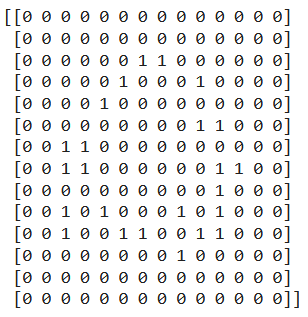
\includegraphics[width=0.4\textwidth]{final_output.png}
    \caption{Final hit-or-miss transformation result (14×14 array)}
    \label{fig:final}
\end{figure}

\section{Technical Explanations}

\subsection{Hit-or-Miss Transform}
\begin{itemize}
    \item \textbf{Purpose}: Detects specific patterns in binary images
    \item \textbf{Kernel Types}: Uses both positive (1) and negative (-1) values to match patterns
    \item \textbf{Condition Sum}: Threshold for successful pattern detection
    \item \textbf{Combination}: Results from multiple kernels are combined using logical OR
\end{itemize}

\subsection{Implementation Notes}
\begin{itemize}
    \item Image converted to (-1, 1) values for pattern matching
    \item Each kernel detects different corner/edge configurations
    \item Boundary pixels are ignored in processing
    \item Final result shows all detected pattern locations
\end{itemize}

\begin{center}
    \href{https://github.com/AsadiAhmad/Hit-and-Miss}{
        \includegraphics[width=0.2\textwidth]{github_logo.png} \\
        \texttt{https://github.com/AsadiAhmad/Hit-and-Miss}
    }
\end{center}

\end{document}